\documentclass[10pt,twocolumn,letterpaper]{article}

\usepackage{cvpr}
\usepackage{times}
\usepackage{epsfig}
\usepackage{graphicx}
\usepackage{amsmath}
\usepackage{amssymb}

\usepackage{url}
\usepackage{listings}
\usepackage{xcolor}

\lstset{
  language=C++,
  basicstyle=\ttfamily\small,
  keywordstyle=\color{orange},
  commentstyle=\color{green!50!black},
  stringstyle=\color{red},
  numbers=left,
  numberstyle=\tiny\color{gray},
  breaklines=true,
  frame=single,
}

% Include other packages here, before hyperref.

% If you comment hyperref and then uncomment it, you should delete
% egpaper.aux before re-running latex.  (Or just hit 'q' on the first latex
% run, let it finish, and you should be clear).
%\usepackage[pagebackref=true,breaklinks=true,letterpaper=true,colorlinks,bookmarks=false]{hyperref}

\cvprfinalcopy % *** Uncomment this line for the final submission

\def\cvprPaperID{****} % *** Enter the CVPR Paper ID here
\def\httilde{\mbox{\tt\raisebox{-.5ex}{\symbol{126}}}}

% Pages are numbered in submission mode, and unnumbered in camera-ready
\ifcvprfinal\pagestyle{empty}\fi
\begin{document}

%%%%%%%%% TITLE
\title{KMeans OpenMP}

\author{Mattia Baroncelli\\
7166468\\
{\tt\small mattia.baroncelli@edu.unifi.it}
% For a paper whose authors are all at the same institution,
% omit the following lines up until the closing ``}''.
% Additional authors and addresses can be added with ``\and'',
% just like the second author.
% To save space, use either the email address or home page, not both
}

\maketitle
\thispagestyle{empty}

%%%%%%%%% ABSTRACT
\begin{abstract}
   Il progetto si concentra sull'implementazione dell'algoritmo K-Means, in particolare il confronto fra la versione sequenziale e quella parallela. K-Means è un algoritmo per l'apprendimento non supervisionato, che permette dato un insieme di punti appartenenti ad uno stesso spazio dimensionale e un valore K, di partizionare l'insieme di punti in K diversi cluster. K-Means crea i cluster assegnando ad ogni punto il centroide più vicino, andando così a minimizzare la varianza all'interno di ogni gruppo. Lo scopo principale del progetto è quindi di implementare una versione parallela dell'algoritmo tramite il framework OpenMP, valutando i vantaggi rispetto alla versione sequenziale. Si andrà inoltre a ricercare la migliore soluzione al problema della parallelizzazione.
\end{abstract}

%%%%%%%%% BODY TEXT
\noindent\textbf{Future Distribution Permission}\\
\indent The author(s) of this report give permission for this document to be distributed to Unifi-affiliated students taking future courses.

\section{Introduction}

L'algoritmo K-Means è un metodo che permette di formare cluster a partire da un dato insieme di punti. Questo viene fatto dando in input all'algoritmo un dataset di punti e un valore K che rappresenta il numero di cluster in cui saranno divisi i punti. L'algoritmo si basa sull'utilizzo dei centroidi, ossia K punti appartenenti al dataset, che durante l'esecuzione dell'algoritmo si andranno a spostare in base all'assegnazione dei punti del dataset ad ogni cluster. Al termine dell'algoritmo ogni punto sarà assegnato al cluster che minimizza la distaza con il proprio centroide. L'algoritmo è composto da tre fasi che vedremo nella prossima sezione ed è un algoritmo molto noto in letteratura, poichè nonostante la sua semplicità nell'implementazione risulta essere molto efficace. Nonostante questo però presenta alcune criticità, infatti all'aumentare della dimensionalità dei punti selezionati, sia per quanto riguarda il numero che per lo spazio, i tempi di esecuzione si dilatano notevolmente. Con lo scopo di superare queste limitazioni ho implementato la versione parallela dell'algoritmo. 
Attraverso il framework \textit{OpenMP} è possibile parallelizzare parte del codice, e tramite questo andremo a valutare quanto l'impatto della parallelizzazione migliori le prestazioni dell'algoritmo.
\begin{figure}[t]
\begin{center}
   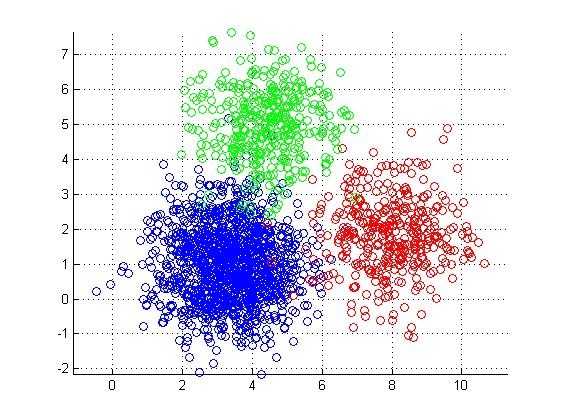
\includegraphics[width=0.8\linewidth]{img1.jpg}
\end{center}
   \caption{Esempio di clustering K-Means con evidenziate le partizioni dei punti.}
\label{fig:kmeans_example}
\end{figure}


%-------------------------------------------------------------------------
\section{Implementazione}
L'algoritmo K-Means è costituito da tre fasi principali, ognuna contraddistinta da step distinti:
\begin{itemize}
   \item Inizializzazione dei centroidi: in questa fase si andranno a selezionare casualmente K punti dal dataset che saranno utilizzati come centroidi.
   \item Assegnamento dei punti ai cluster: l'algoritmo andrà a cercare per ogni punto il centroide a lui più vicino e di conseguenza gli assegnerà il corrispondente cluster.
   \item Aggiornamento dei centroidi: una volta assegnati tutti i punti verrà fatta una media delle posizioni dei punti appartenente ad ogni cluster per aggiornare il relativo centroide.
\end{itemize}
Sull'implementazione di ogni fase ci concentreremo di seguito quando parleremo nel dettaglio del confronto fra versione sequenziale e parallela.
Per quanto riguarda le condizioni di convergenza dell'algoritmo esistono varie scelte, io ho preferito interrompere l'algoritmo quando nessun punto ha cambiato cluster dopo un'iterazione di assegnazione dei punti ai rispettivi gruppi.

\subsection{OpenMP directives}
Prima di iniziare con l'analisi del codice è utile vedere le direttive che andrò ad utilizzare per parallelizzare l'algoritmo nel progetto. Grazie a questo particolare tipo di istruzioni presenti in \textit{OpenMP} è possibile creare multipli threads così da velocizzare l'esecuzione del codice, di seguito le direttive che ho usato. 
\begin{itemize}
   \item \lstinline{#pragma omp parallel}: Grazie a questa istruzione è possibile generare multipli threads all'interno del programma.
   \item \lstinline{#pragma omp for} : the \textit{omp for} directive instructs the compiler to distribute loop iterations within the team of threads that encounters this work-sharing construct.
   \item \lstinline{#pragma omp critical}: The \textit{omp critical} directive identifies a section of code that must be executed by a single thread at a time.
\end{itemize}
Grazie a queste direttive non solo riusciremo a parallelizzare il codice, ma anche ad evitare problemi che potrebbero nascere proprio a causa della parallelizzazione.

\subsection{Sequential version}
Iniziamo l'analisi con la versione sequenziale dell'algoritmo K-Means. L'algoritmo è molto noto in letteratura e come detto prima è formato da tre parti principali. L'algoritmo è stato scritto in modo tale da potersi adattare alla versione parallela con poche aggiunte (principalmente le direttive \textit{OpenMP}).

\begin{lstlisting}[caption={Fase di assegnamento della versione sequenziale}, label={lst:openmp}]
for (int i = 0; i < n; i++) {  
   double min_dist = std::numeric_limits<double>::max(); 
   int best_cluster = -1; 

   for (int j = 0; j < K; ++j) { 
         double dist = calculateDistanceSquare(points[i].values, centroids[j]);  
         if (dist < min_dist) { 
            min_dist = dist;  
            best_cluster = j;    
         }
   }
   if (points[i].cluster != best_cluster) {
         points[i].cluster = best_cluster;
         changed = true; 
   }
}
\end{lstlisting}

Il primo blocco di codice che andiamo ad analizzare riguarda la fase di assegnamento di ogni punto al proprio centroide. La fase di selezione dei centroidi, infatti, non è molto interessante per l'analisi e quindi abbiamo preferito non riportarla.
Nel codice si andrà ad effettuare un ciclo per ogni punto e per ogni centroide si andrà a calcolare la distanza fra quest'ultimo e il punto, andando di volta in volta ad aggiornare il parametro \lstinline{min_dist} fino a trovare il centroide che minimizza la distanza con il punto selezionato. Infine se il centroide ha cambiato cluster, si và ad aggiornare il cluster e a cambiare il valore di un flag necessario per verificare la condizione di arresto. Andiamo adesso a vedere la parte del codice che riguarda il calcolo dei nuovi centroidi.

\begin{lstlisting}[caption={Fase di aggiornamento dei centroidi della versione sequenziale}, label={lst:openmp}]
std::vector<std::vector<double>> new_centroids_sum(K, std::vector<double>(dimensions, 0.0));   
        std::vector<int> cluster_counts(K, 0);  
for (int i = 0; i < n; ++i) {   
   int cluster_id = points[i].cluster;     
   cluster_counts[cluster_id]++;       
   for (int d = 0; d < dimensions; ++d) {  
         new_centroids_sum[cluster_id][d] += points[i].values[d];  
         }
}

for (int j = 0; j < K; ++j) {   
   if (cluster_counts[j] > 0) {
         for (int d = 0; d < dimensions; ++d) {
            centroids[j][d] = new_centroids_sum[j][d] / cluster_counts[j];
         }
   }
}
\end{lstlisting}

In questo blocco vengono innanzitutto inizializzati due parametri: una matrice che si occuperà di conservare le somme dei punti che appartengono ad un particolare centroide per ognuna delle sue dimensioni e un vettore che conta il numero di punti all'interno di un cluster.
Si ha quindi un ciclo su ogni punto, che andrà ad incrementare il contatore del relativo cluster e andrà ad aggiornare la matrice delle somme.
Una volta aggiornati questi due parametri per ogni punto si andrà ad effettuare la media dividendo i valori all'interno della matrice per il vettore delle somme di ogni centroide, ottenendo così le coordinate dei centroidi aggiornate. Senza far vedere il codice ritengo corrette citare la condizione di arresto che si verifica quando dopo un'iterazione dell'algoritmo nessun punto ha cambiato cluster rispetto all'iterazione precedente, ed è implementato con un semplice ciclo \lstinline{while}.


\subsection{Parallel version}
Dopo aver implementato la versione sequenziale del co-
dice vediamo adesso come è possibile passare ad una ver-
sione parallela.
Le versioni parallele sviluppate in realtà sono due, che sfruttano due approcci diversi della parallelizzazione:
\begin{itemize}
   \item Array of Structures (AoS): E' l'approccio più vicino a quanto implementato con la versione sequenziale. I dati sono organizzati in memoria in modo che il singolo punto abbia le proprie coordinate spazialmente vicine.
   \item Structure of Arrays (SoA): Questo approccio separa la singole componenti dei punti in array distinti, permettendo ai thread di leggere blocchi contigui di memoria durante il calcolo delle distanze.
\end{itemize}
A livello teorico quindi l'approccio SoA dovrebbe darci risultati migliori in termini di speed-up rispetto alla versione sequenziale, vedremo nella sezione degli Esperimenti se questo sarà confermato.
Soffermiamoci adesso ad analizzare entrambe le versioni di codice che abbiamo implementato.

\subsubsection{Array of Structures}
Come detto prima questa prima versione parallela non si discosta molto da quella sequenziale, grazie all'approccio usato in precedenza è sufficiente adattare il codice prestando attenzione ad alcune problemi derivati dalla parallelizzazione.
Andiamo innanzitutto a valutare la struttura della classe \lstinline{Point}, che risulta esere la stessa utilizzata nella versione sequenziale
\begin{lstlisting}[caption={Implementazione dei punti nella versione AoS}, label={lst:openmp}]
struct Point {
    int cluster;
    std::vector<double> values;

    Point(std::vector<double> v);
};
\end{lstlisting}
Ogni punto è quindi formato dalle proprie coordinate di appartenenza e dall'ID del proprio cluster, che è inizializzato a -1 nella fase di inizializzazione dei punti.
Andiamo quindi adesso ad analizzare il codice che assegna i punti ai cluster

\begin{lstlisting}[caption={Fase di assegnamento parallela AoS}, label={lst:openmp}]
#pragma omp parallel for reduction(||:changed)
for (int i = 0; i < n; i++) {
   double min_dist = std::numeric_limits<double>::max();
   int best_cluster = -1;

   for (int j = 0; j < K; ++j) {
         double dist = calculateDistanceSquare(points[i].values, centroids[j]);
         if (dist < min_dist) {
            min_dist = dist;
            best_cluster = j;
         }
   }

   if (points[i].cluster != best_cluster) {
         points[i].cluster = best_cluster;
         changed = true;
   }
}
\end{lstlisting}

All'atto pratico il codice risulta essere uguale alla versione sequenziale, con l'aggiunta della direttiva \lstinline{#pragma omp parallel for reduction(||:changed)}, il costrutto serve a parallelizzare il ciclo for sottostante che effettua il calcolo delle distanze fra punti e centroidi e assegna ogni punto a un centroide, in questo caso le variabili \lstinline{min_dist} e \lstinline{best_cluster} venendo dichiarate all'interno del ciclo diventano private per il thread che sta eseguendo. Lo stesso non si può dire del flag \lstinline{changed} che viene inizializzato fuori dal ciclo e che può portare ad un comportamento indefinito. Se due thread cercano di scrivere nello stesso momento in quella cella di memoria possono verificarsi rallentamenti o nella peggiore delle ipotesi la corruzione del dato e di conseguenza un funzionamento errato dell'algoritmo (potrebbe fermarsi prima). Per risolvere questo problema utilizziamo il costrutto reduction. OpenMP andrà a creare delle copie locali della variabile \lstinline{changed}. Una volta terminato il ciclo OpenMP fonde le variabili locali tramite l'operatore OR (che gli abbiamo passato). Il risultato pertanto sarà lo stesso ma evitando il problema citato in precedenza.


\begin{lstlisting}[caption={Fase di aggioramento dei centroidi parallela AoS}, label={lst:openmp}]
#pragma omp parallel
        {
std::vector<std::vector<double>> local_centroids_sum(K, std::vector<double>(dimensions, 0.0));
std::vector<int> local_cluster_counts(K, 0);

#pragma omp for
for (int i = 0; i < n; ++i) {
      int cluster_id = points[i].cluster;
      local_cluster_counts[cluster_id]++;
      for (int d = 0; d < dimensions; ++d) {
         local_centroids_sum[cluster_id][d] += points[i].values[d];
      }
}


#pragma omp critical
{
      for (int j = 0; j < K; ++j) {
         cluster_counts[j] += local_cluster_counts[j];
         for (int d = 0; d < dimensions; ++d) {
            new_centroids_sum[j][d] += local_centroids_sum[j][d];
         }
      }
}
} 

for (int j = 0; j < K; ++j) {
if (cluster_counts[j] > 0) {
      for (int d = 0; d < dimensions; ++d) {
         centroids[j][d] = new_centroids_sum[j][d] / cluster_counts[j];
      }
}
}
\end{lstlisting}

La fase di aggiornamento dei centroidi i apre con, oltre alla dichiarazione degli accumulatori di somme e numero di punti, anche con quella di accumulatori locali per ogni cluster, che assegneremo ad ogni thread. Anche stavolta tramite la direttiva \lstinline{#pragma omp for}, andremo a parallelizzare il ciclo. In manier analoga a prima ogni thread andrà ad aggiornare i propri accumulatori. Una volta terminato l'aggiornamento degli accumulatori per ogni punto, è necessario aggiornare gli accumulatori globali, andandogli ad assegnare la somma dei rispettivi contatori parziali. Questa operazione può portare al verificarsi di una race condition, dove due threads leggono un valore e provano a sovrascrivere gli accumulatori globali con i propri valori, rischiando di portare a risultati errati. Per risolvere questo problema abbiamo adottato il costrutto \lstinline{#pragma omp critical} che assicura che un solo thread alla volta aggiorni i contatori globali.

\subsubsection{Structure of Arrays}
Andiamo a vedere in questa sezione come è possibile implementare l'algoritmo con il paradigma SoA. Di seguito il codice che illustra la struttura l'implementazione dei punti con questa tecnica.

\begin{lstlisting}[caption={struct \textit Implementazione dei punti nella versione SoA}, label={lst:openmp}]
struct DatasetSoA {
    int num_points;
    int dimensions;
   
    std::vector<double> coords; 
    std::vector<int> clusters;  
};

\end{lstlisting}

Il dataset viene implementato tramite la struct DatasetSoA che ha come attributi, il numero totale di punti e di dimensioni, il vettore che rappresenta le coordinate dei punti e un array separato per etichette dei clusters. La funzione \lstinline{convertToSoA} si occuperà di convertire i punti passati nel formato AoS, in questo formato, tramite un ciclo for. 

\begin{lstlisting}[caption={ciclo for all'interno di convertToSoA}, label={lst:openmp}]
for (int i = 0; i < soa.num_points; ++i) {
   soa.clusters[i] = aos_dataset[i].cluster;
   for (int d = 0; d < soa.dimensions; ++d) {
      // Indice piatto: (riga * numero_colonne) + colonna
      soa.coords[i * soa.dimensions + d] = aos_dataset[i].values[d];
   }
}
\end{lstlisting}

In particolare la funzione prende in input il dataset in formato AoS e innanzitutto assegna il medesimo cluster di ogni punto alla rappresentazione in formato SoA, successivamente attraverso la tecnica del flat index, costruisce l'array di coordinate. In questo modo è possibile passare facilmente dalla rappresentazione AoS a SoA. Anche l'algoritmo avrà necessità di essere adattato, in particolare, oltre a una diversa versione dell'algoritmo per calcolare la distanza, che sfrutta anch'esso il flat index; abbiamo una differenza sostanziale nella terza fase dell'algoritmo.

\begin{lstlisting}[caption={Fase di aggioramento dei centroidi SoA}, label={lst:openmp}]
std::vector<double> new_centroids_sum(K * dims, 0.0);
std::vector<int> cluster_counts(K, 0);

#pragma omp parallel
{
std::vector<double> local_centroids_sum(K * dims, 0.0);
std::vector<int> local_cluster_counts(K, 0);

for (int i = 0; i < n; ++i) {
   int cluster_id = dataset.clusters[i];
   local_cluster_counts[cluster_id]++;
   
   for (int d = 0; d < dims; ++d) {
      local_centroids_sum[cluster_id * dims + d] += dataset.coords[i * dims + d];
   }
}

{
   for (int j = 0; j < K; ++j) {
      cluster_counts[j] += local_cluster_counts[j];
      for (int d = 0; d < dims; ++d) {
         new_centroids_sum[j * dims + d] += local_centroids_sum[j * dims + d];
      }
   }
}
} 

for (int j = 0; j < K; ++j) {
if (cluster_counts[j] > 0) {
   for (int d = 0; d < dims; ++d) {
      centroids[j * dims + d] = new_centroids_sum[j * dims + d] / cluster_counts[j];
   }
}
}
\end{lstlisting}

Nelle operazioni compiute il codice è molto simile a quello scritto per la versione AoS. Fin da subito però è possibile notare come sia gli accumulatori globali che quelli locali siano cambiate. In questa versione infatti si richiede per le somme dei centroidi una allocazione per un blocco continuo, al contrario delle metrici allocate in precedenza. Inoltre il costrutto di parallelizzazione è diventato \lstinline{#pragma omp for schedule(static)}, che forza l'assegnazione dei blocchi contigui ad uno stesso thread (cosa che è stata aggiunta anche alla fase di assegnamento dei punti). Infine sia il calcolo della somma dei centroidi e della media finale vengono fatte utilizzando la rappresentazione piatta.











%-------------------------------------------------------------------------

\section{Esperimenti}
Iniziamo adesso la sezione del report che riguarda gli
esperimenti effettuati, abbiamo visto come i tre diversi tipi
di implementazione variano a livello di codice, adesso vediamo quanto variano a livello di prestazioni. Per farlo è necessario partire innanzitutto dalla creazione del dataset.

\subsection{Dataset}
I dataset sono stati creati attraverso una funzione Python creata appositamente \lstinline{generate_dataset}. La funzione prende in input:
\begin{itemize}
   \item Numero di punti (N)
   \item Numero di cluster (K)
   \item Dimensione del piano su cui giaccioni i punti
   \item Parametro di dispersione dei punti
\end{itemize}
e restituisce in output un dataset in formato csv, che contiene sulle righe le coordinate di ogni punto. Poichè k-means è un algoritmo non supervisionato nel dataset non è presente il cluster di appartenenza, nonostante ciò il numero di cluster è un parametro in input per creare dataset che abbiamo punti che vadano a formare cluster definiti. Per convertire i punti in formato SoA verrà poi usata la funzione apposita definita nella sezione precedente; la conversione come era logico aspettarsi non concorrerà alla misurazione del tempo di esecuzione dell'algoritmo.


\subsection{Aumento N AoS}
%COme variabili ho K,N, numCore, AosSoA, Tempo/SPeedup
Iniziamo quindi gli esperimenti valutando le prestazione della tecnica Structure of Arrays su vari dataset. Il primo esperimento verrà fatto aumentando la dimensione del numero di punti (N), mantendendo fermo il numero di cluster K a 10. Andremo inoltre ad aumentare gradualmente il numero threads in esecuzione, per verificare se c'è un miglioramento delle performace all'aumentare dei threads.

%Grafico speed up x:numthreads y:speedup colorato:dimdataset

\subsection{Aumento K}








%----------------------------------------------------------
\section{Conclusioni}
%----------------------------------------------------------
\subsection{The ruler}


\subsection{Mathematics}

Please number all of your sections and displayed equations.  It is
important for readers to be able to refer to any particular equation.  Just
because you didn't refer to it in the text doesn't mean some future reader
might not need to refer to it.  It is cumbersome to have to use
circumlocutions like ``the equation second from the top of page 3 column
1''.  (Note that the ruler will not be present in the final copy, so is not
an alternative to equation numbers).  All authors will benefit from reading
Mermin's description of how to write mathematics: \url{http://www.cvpr.org/doc/mermin.pdf}.

\subsection{Miscellaneous}

\noindent
Compare the following:\\
\begin{tabular}{ll}
 \verb'$conf_a$' &  $conf_a$ \\
 \verb'$\mathit{conf}_a$' & $\mathit{conf}_a$
\end{tabular}\\
See The \TeX book, p165.

The space after \eg, meaning ``for example'', should not be a
sentence-ending space. So \eg is correct, {\em e.g.} is not.  The provided
\verb'\eg' macro takes care of this.

When citing a multi-author paper, you may save space by using ``et alia'',
shortened to ``\etal'' (not ``{\em et.\ al.}'' as ``{\em et}'' is a complete word.)
However, use it only when there are three or more authors.  Thus, the
following is correct: ``
   Frobnication has been trendy lately.
   It was introduced by Alpher~\cite{Alpher02}, and subsequently developed by
   Alpher and Fotheringham-Smythe~\cite{Alpher03}, and Alpher \etal~\cite{Alpher04}.''

This is incorrect: ``... subsequently developed by Alpher \etal~\cite{Alpher03} ...''
because reference~\cite{Alpher03} has just two authors.  If you use the
\verb'\etal' macro provided, then you need not worry about double periods
when used at the end of a sentence as in Alpher \etal.

For this citation style, keep multiple citations in numerical (not
chronological) order, so prefer \cite{Alpher03,Alpher02,Authors06} to
\cite{Alpher02,Alpher03,Authors06}.


\begin{figure*}
\begin{center}
\fbox{\rule{0pt}{2in} \rule{.9\linewidth}{0pt}}
\end{center}
   \caption{Example of a short caption, which should be centered.}
\label{fig:short}
\end{figure*} 

%------------------------------------------------------------------------
\section{Formatting your paper}

All text must be in a two-column format. The total allowable width of the
text area is $6\frac78$ inches (17.5 cm) wide by $8\frac78$ inches (22.54
cm) high. Columns are to be $3\frac14$ inches (8.25 cm) wide, with a
$\frac{5}{16}$ inch (0.8 cm) space between them. The main title (on the
first page) should begin 1.0 inch (2.54 cm) from the top edge of the
page. The second and following pages should begin 1.0 inch (2.54 cm) from
the top edge. On all pages, the bottom margin should be 1-1/8 inches (2.86
cm) from the bottom edge of the page for $8.5 \times 11$-inch paper; for A4
paper, approximately 1-5/8 inches (4.13 cm) from the bottom edge of the
page.

%-------------------------------------------------------------------------
\subsection{Margins and page numbering}

All printed material, including text, illustrations, and charts, must be
kept within a print area 6-7/8 inches (17.5 cm) wide by 8-7/8 inches
(22.54 cm) high.


%-------------------------------------------------------------------------
\subsection{Type-style and fonts}

Wherever Times is specified, Times Roman may also be used. If neither is
available on your word processor, please use the font closest in
appearance to Times to which you have access.

MAIN TITLE. Center the title 1-3/8 inches (3.49 cm) from the top edge of
the first page. The title should be in Times 14-point, boldface type.
Capitalize the first letter of nouns, pronouns, verbs, adjectives, and
adverbs; do not capitalize articles, coordinate conjunctions, or
prepositions (unless the title begins with such a word). Leave two blank
lines after the title.

AUTHOR NAME(s) and AFFILIATION(s) are to be centered beneath the title
and printed in Times 12-point, non-boldface type. This information is to
be followed by two blank lines.

The ABSTRACT and MAIN TEXT are to be in a two-column format.

MAIN TEXT. Type main text in 10-point Times, single-spaced. Do NOT use
double-spacing. All paragraphs should be indented 1 pica (approx. 1/6
inch or 0.422 cm). Make sure your text is fully justified---that is,
flush left and flush right. Please do not place any additional blank
lines between paragraphs.

Figure and table captions should be 9-point Roman type as in
Figures~\ref{fig:onecol} and~\ref{fig:short}.  Short captions should be centred.

\noindent Callouts should be 9-point Helvetica, non-boldface type.
Initially capitalize only the first word of section titles and first-,
second-, and third-order headings.

FIRST-ORDER HEADINGS. (For example, {\large \bf 1. Introduction})
should be Times 12-point boldface, initially capitalized, flush left,
with one blank line before, and one blank line after.

SECOND-ORDER HEADINGS. (For example, { \bf 1.1. Database elements})
should be Times 11-point boldface, initially capitalized, flush left,
with one blank line before, and one after. If you require a third-order
heading (we discourage it), use 10-point Times, boldface, initially
capitalized, flush left, preceded by one blank line, followed by a period
and your text on the same line.

%-------------------------------------------------------------------------
\subsection{Footnotes}

Please use footnotes\footnote {This is what a footnote looks like.  It
often distracts the reader from the main flow of the argument.} sparingly.
Indeed, try to avoid footnotes altogether and include necessary peripheral
observations in
the text (within parentheses, if you prefer, as in this sentence).  If you
wish to use a footnote, place it at the bottom of the column on the page on
which it is referenced. Use Times 8-point type, single-spaced.


%-------------------------------------------------------------------------
\subsection{References}

List and number all bibliographical references in 9-point Times,
single-spaced, at the end of your paper. When referenced in the text,
enclose the citation number in square brackets, for
example~\cite{Authors06}.  Where appropriate, include the name(s) of
editors of referenced books.

\begin{table}
\begin{center}
\begin{tabular}{|l|c|}
\hline
Method & Frobnability \\
\hline\hline
Theirs & Frumpy \\
Yours & Frobbly \\
Ours & Makes one's heart Frob\\
\hline
\end{tabular}
\end{center}
\caption{Results.   Ours is better.}
\end{table}

%-------------------------------------------------------------------------
\subsection{Illustrations, graphs, and photographs}

All graphics should be centered.  Please ensure that any point you wish to
make is resolvable in a printed copy of the paper.  Resize fonts in figures
to match the font in the body text, and choose line widths which render
effectively in print.  Many readers (and reviewers), even of an electronic
copy, will choose to print your paper in order to read it.  You cannot
insist that they do otherwise, and therefore must not assume that they can
zoom in to see tiny details on a graphic.

When placing figures in \LaTeX, it's almost always best to use
\verb+\includegraphics+, and to specify the  figure width as a multiple of
the line width as in the example below
{\small\begin{verbatim}
   \usepackage[dvips]{graphicx} ...
   \includegraphics[width=0.8\linewidth]
                   {myfile.eps}
\end{verbatim}
}


%-------------------------------------------------------------------------
\subsection{Color}

Color is valuable, and will be visible to readers of the electronic copy.
However ensure that, when printed on a monochrome printer, no important
information is lost by the conversion to grayscale.

{\small
\bibliographystyle{ieee}
\bibliography{egbib}
}

\section{Appendix}
If your course project is part of a larger project from another class or research lab, please fill in this section and clearly spell out the following items:

\begin{enumerate}
\item  Explicitly explain what the computer vision components are in this course project;
\item  Explicitly list out all of your own contributions in this project in terms of:
	\begin{enumerate}
	\item ideas
	\item formulations of algorithms
 	\item software and coding
	\item designs of experiments
	\item analysis of experiments
	\end{enumerate}
\item Verify and confirm that you (and your partner currently taking CS231A) are the sole author(s) of the writeup.
Please provide papers, theses, or other documents related to this project so that we can compare with your own writeup.
\end{enumerate}
\end{document}
